
\chapter{Grafos gerados referentes ao \emph{ResourceManager}}

%IMPORTANTE: Se precisar usar alguma seção ou subseção dentro dos apêndices ou
%anexos, utilizar o comando \tocless para não adicionar no Sumário
%Exemplos: 
% \tocless\section{Histórico}
% \tocless\subsection{Detalhes}
%\tocless\section{teste}
%Este é um teste de seção dentro do apêndice

\begin{figure}[hbtn]
   \centering
   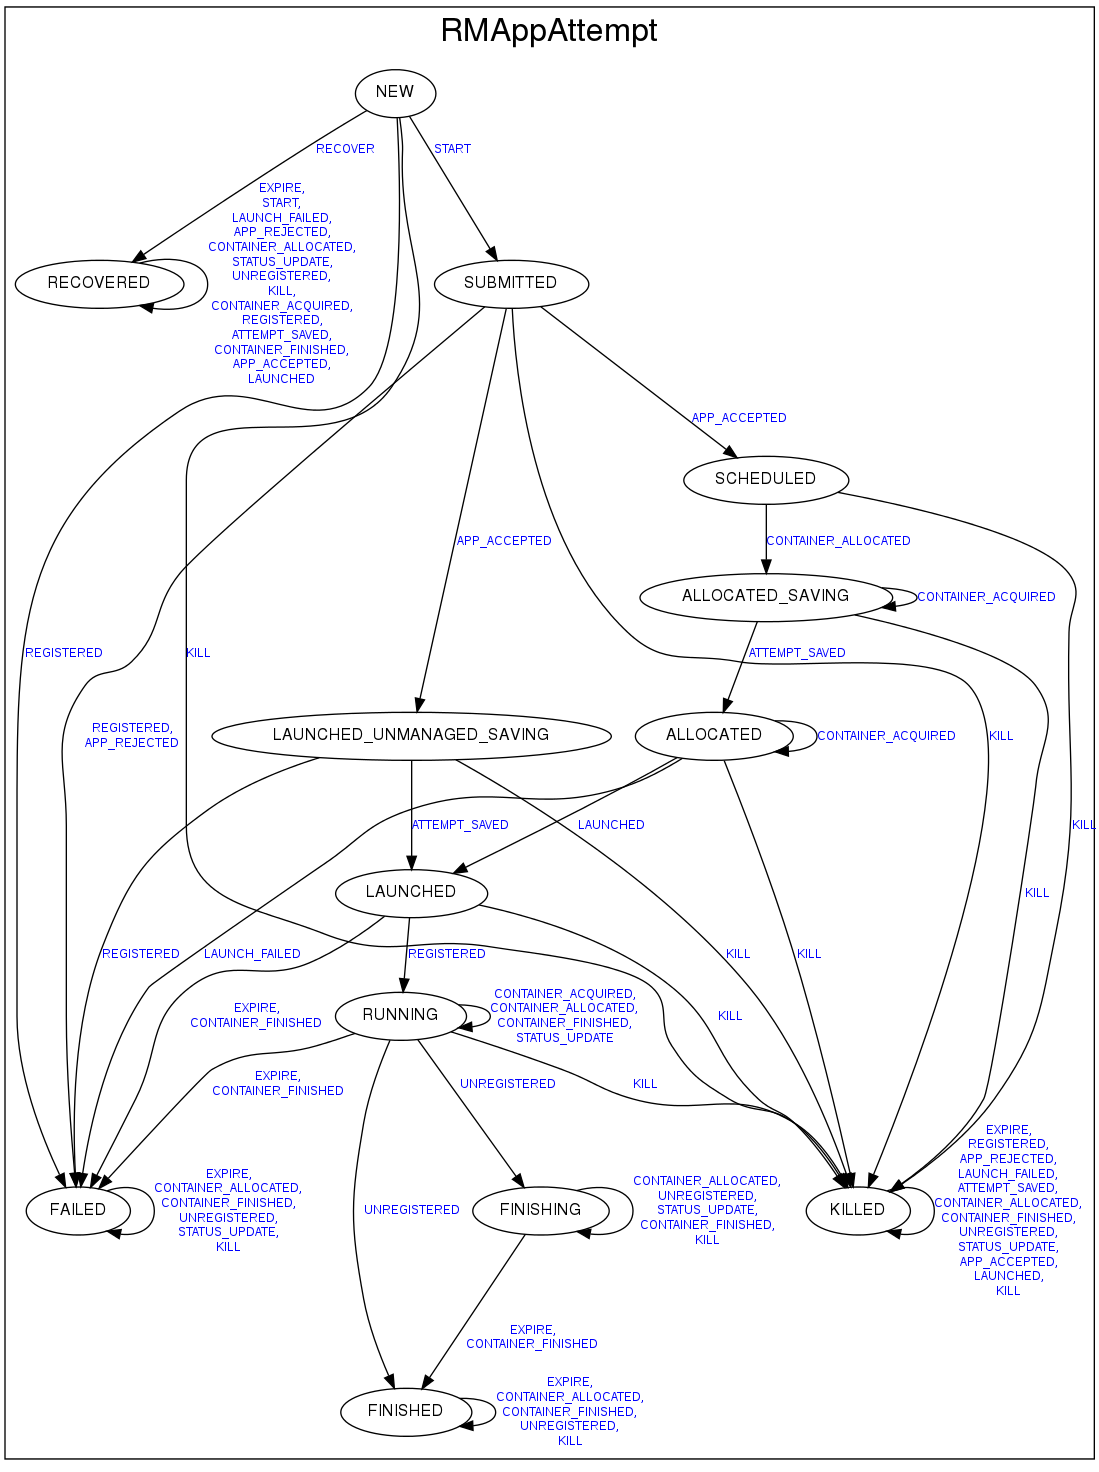
\includegraphics[width=15cm]{figuras/Figura02-RMAppAttempt.png}
   \caption{Máquina de estados do RMAppAttempt}
   \label{fig:RMAppAttempt}
\end{figure}

\begin{figure}[hbtn]
   \centering
   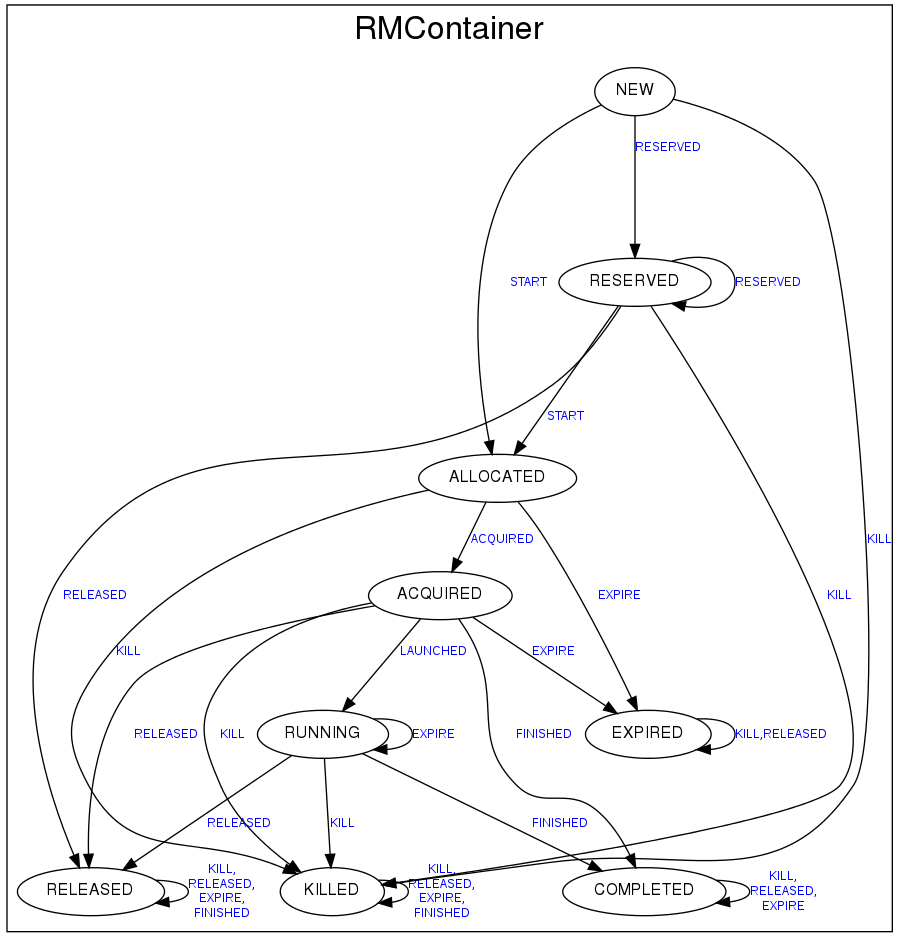
\includegraphics[width=15cm]{figuras/Figura03-RMContainer.png}
   \caption{Máquina de estados do RMContainer}
   \label{fig:RMContainer}
\end{figure}

\begin{figure}[hbtn]
   \centering
   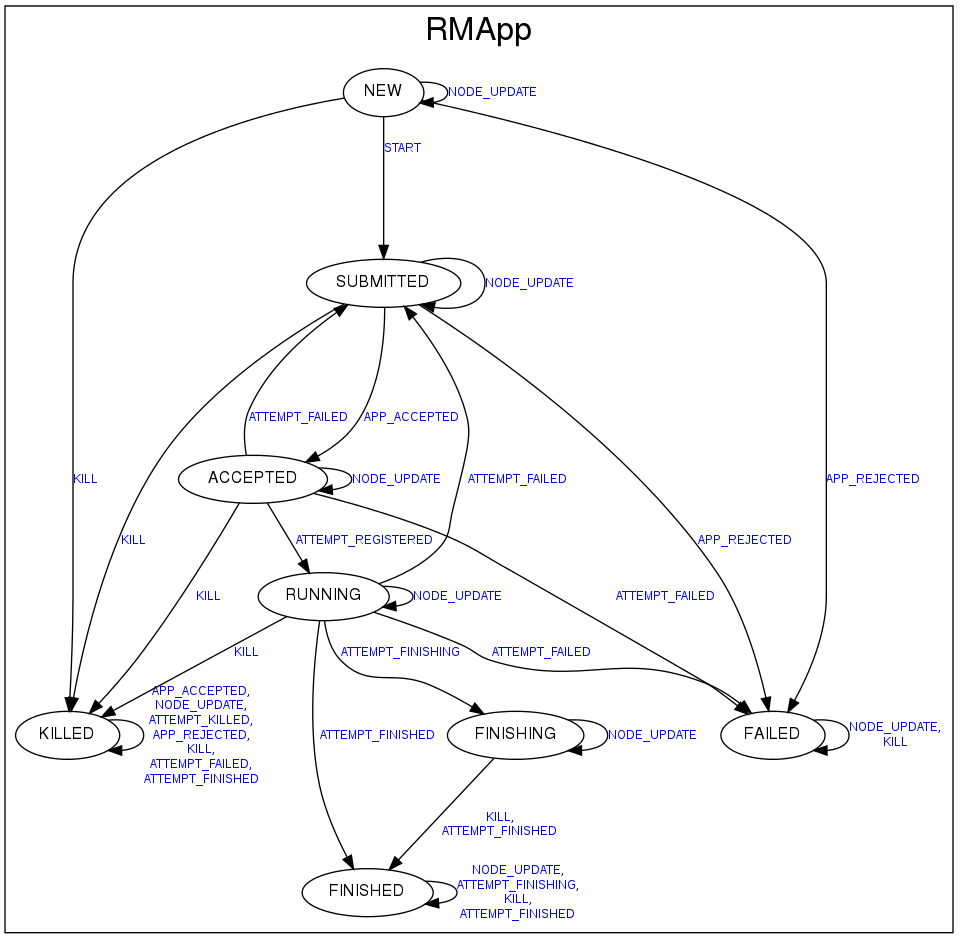
\includegraphics[width=15cm]{figuras/Figura04-RMApp.png}
   \caption{Máquina de estados do RMApp}
   \label{fig:RMApp}
\end{figure}

\begin{figure}[hbtn]
   \centering
   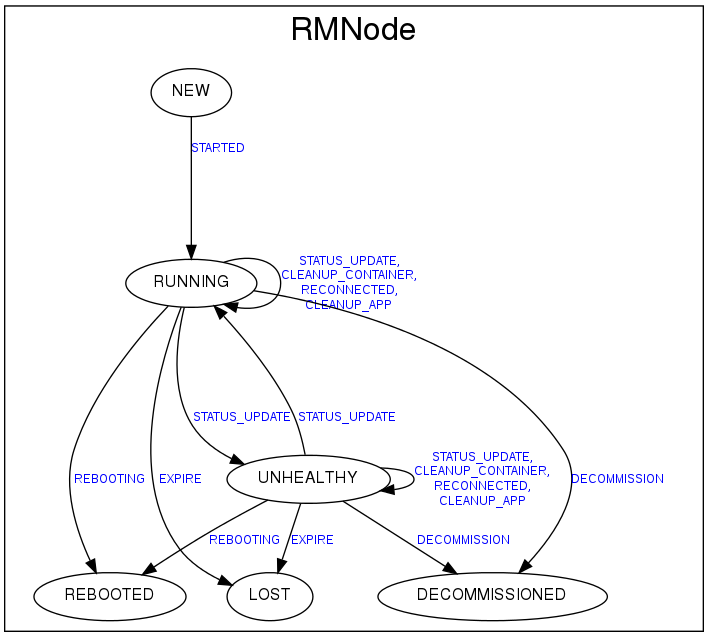
\includegraphics[width=15cm]{figuras/Figura05-RMNode.png}
   \caption{Máquina de estados do RMNode}
   \label{fig:RMNode}
\end{figure}

